\documentclass[10pt,letterpaper]{article}
\usepackage{fullpage}
\usepackage{xcolor}
\usepackage[top=1in, bottom=1in, left=1in, right=1in]{geometry}
\usepackage{graphicx}
\usepackage{wrapfig}
\usepackage{hyperref}
\usepackage{booktabs}
\usepackage{multirow}

\newcommand{\todo}[1]{\textcolor{red}{TODO:\ #1}}
\newcommand{\shortname}{EqMap}

\title{ECE6745 Project Proposal}
\author{Matthew Hofmann}
\date{\today}

\begin{document}

\maketitle

% Revised Sections
% Introduction
% Background (lit review)
% Baseline design

\section{Introduction}\label{sec:intro}
\subsection{Motivation}\label{sec:intro:motivation}

As the trends of transistor scaling come to a close, the QoR (quality of
results) of EDA tools will become more of a bottleneck in the hardware design
process. Given new developments in compiler technology and automated reasoning
tools, it is possible to better study the suboptimality of the EDA tool stack.
Several of the heuristics used in core EDA algorithms were invented decades
ago, and increases in compute capacity in the modern era afford us a more
formal and exploratory approach to optimizing digital logic. In this project, I
use the automated reasoning capabilities of equality graphs (e-graphs) to more
precisely explore optimal designs points in the PPA (power, performance, area)
trade-off space. With my results, I demonstrate that e-graph driven compilers
can better span the wide gap between SAT-based, exact synthesis and fully
heuristic algorithms.

\subsection{Project Proposal}\label{sec:intro:proposal}

Over the length of this course project, I have developed a tool which uses
e-graphs to superoptimize ASIC technology mapping. Besides developing the core
optimization and mapping framework, I have developed a Verilog parser and
emitter to be able to test my technique against existing RTL tools. In short, I
will be comparing against Synopsys Design Compiler. Across 96 RTL benchmarks,
my tool, called \shortname{}, should be able to more exactly synthesize
combinational logic to standard cells. My goal is roughly 10\% area savings
without increasing the circuit depth.

I am optimistic tat my tool can outperform Synopsys on small designs, because
e-graphs can explore circuit topologies that heuristic methods cannot. However,
the real challenge may lie in the extraction algorithm. For this reason, I will
also consider optimizing for delay if that proves to be more feasible than
optimizing for area. All of these experiments were relatively low cost to
start, because I have a lot of compiler infrastructure already built up. For
instance, I have a custom, bare-bones Verilog frontend. In the following
sections, I will give the literature review needed to understand equality
graphs for superoptimization as well as ASIC technology mapping in general.

\section{Literature Review}\label{sec:background}

\subsection{E-Graphs}\label{sec:background:egraph}

Equality graphs, most commonly referred to as \textit{e-graphs}, are an
automated reasoning tool built around a union-find data
structure~\cite{eggpaper}. An e-graph is essentially a directed graph with two
extra features: (1) nodes are grouped together into \textit{e-classes} and (2)
edges always start at a node and point to an e-class. As a consequence,
e-graphs can very compactly store a collection of equivalence relations. The
prototypical example for e-graphs involves the rewriting of arithmetic
expressions. For instance, one relation conveyed in Fig.~\ref{fig:egraph} is
that \texttt{a << 1} is equal to \texttt{a * 2}. To convey equality, the
anchoring nodes \texttt{<<} and \texttt{*} are grouped in the same e-class (the
dotted box). However, it is important to note that the destination of edges is
always an e-class and not a node. With this illustration, it hopefully becomes
clear why e-graphs are strong at equational reasoning.

\begin{wrapfigure}{r}{0.47\textwidth}
    \centering
    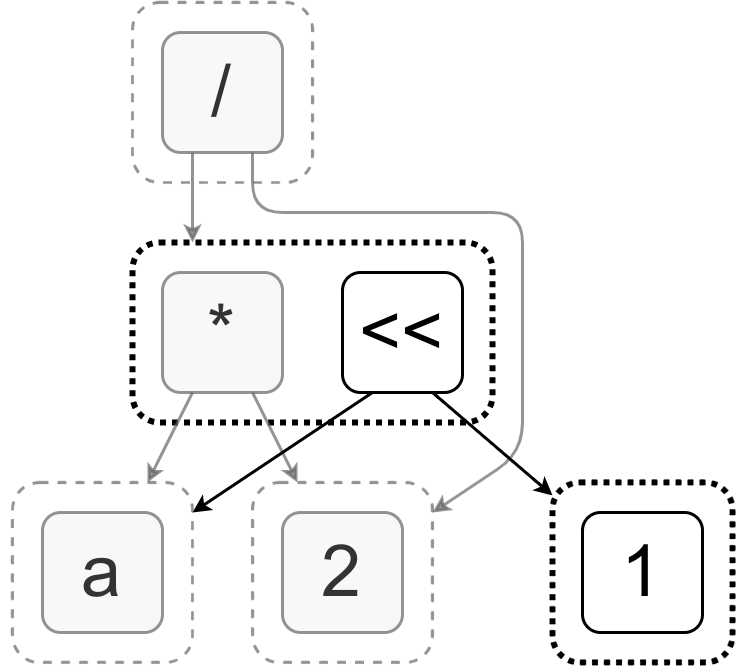
\includegraphics[width=0.44\textwidth]{img/egraph.png}
    \caption{An e-graph with 5 e-classes and 6 e-nodes.}\label{fig:egraph}
\end{wrapfigure}

To give some practical examples, e-graphs have been used to rewrite
mathematical expressions~\cite{egraphmath} or for automated reasoning about
functional programs~\cite{cclemma}. In the case of EDA software, e-graphs can
drive logic synthesis by exploring other circuit topologies. Initially, each
circuit node starts alone in its equivalence class. Then, a set of rewrite
rules is used to grow the e-graph with alternative representations. When
rewrite rules no longer introduce new information into the graph, we say we
have reached \textit{equality saturation}.

Of course, optimizing technology mapping for area is still an NP-hard problem.
E-graphs defer the difficult problem of finding the `best' circuit into a phase
called \textit{extraction}. This is where heuristics are re-introduced. There
are several research projects on e-graph
extraction~\cite{smoothe,sparsextract}, but they are beyond the scope of this
course project. However, previous work on FPGA technology mapping has
demonstrated that fast, greedy extraction algorithms can be used and still find
area and circuit depth improvements. Previous work~\cite{esyn} has demonstrated
the usefulness of e-graphs for logic synthesis. Moreover, I hope to submit my
own e-graph work to ICCAD which shows 12\% area savings over vendor tools on
FPGA applications without increasing circuit depth.

\subsection{ASIC Technology Mapping}\label{sec:background:techmapping}

The standard-cell design methodology for semiconductors came to fruition in the
1980s and 90s. While ASIC design as a general technique is more manageable than
full-custom layouts, there are still provably difficult problems in the flow.
In general, Boolean logic minimization is NP-hard, and this carries over to
more architecture-specific problems, like technology mapping. Technology
mapping is the compilation step which converts the abstract RTL logic into a
network of design elements that belong to the standard cell library. In other
words, the input is the user-written logic and the output is a gate netlist.
Since exact technology mapping is hard, most logic synthesis tools are largely
driven by heuristics---either for minimizing area or delay. For instance,
Lily~\cite{areamap} takes into account the connectivity of a circuit in order
to reduce area dedicated to routing signals. Another is example is
how~\cite{powermap} maps cells while taking into account signal transition
probabilities in order to minimize power. Recent developments include works
that use more approximate methods to drive synthsis. For example,
ALS~\cite{approxmap} uses reinforncement learning to do a form of `lossy' logic
synthesis. In my project, I will mostly perform area optimization by tracking
cell counts.

\section{Baseline Compiler Design}\label{sec:baseline}

In total, I have a collection of 96 RTL benchmarks combined from three academic
sources: ISCAS'85, LGSYNTH'91, and
EPFL\footnote{\href{https://github.com/matth2k/synth-benchmarks}{https://github.com/matth2k/synth-benchmarks}}.
They are mostly combinational benchmarks, but sequential logic can also be
tested. In general, I will consider Synopsys Design Compiler as the baseline
synthesis tool.

\subsection{More Exact Synthesis}
In this experiment, I will develop logic rewriting systems and extraction
techniques that can achieve better results than Synopsys Design Compiler. In
the case of FPGA technology mapping, I already have results that show 12\% area
savings over the vendor tools without degrading timing. Moreover, I already
have a robust Boolean logic rewriting system that can be extended to standard
cell design. However, the potential pitfalls come with extraction technique.
While greedy extraction shows promise for FPGA applications, I have gut
feelings that the same extraction algorithm will not work as well for ASIC
design. ASIC cell mapping appears less like a graph covering algorithm, because
most of the cells have fanin of 1-3. FPGAs, on the other hand, have 6 input
lookup tables. Nonethless, I could be underestimating the flexibility of
standard cell design. Perhaps basic greedy extraction algorithms would still
work for synthesizing to standard cells. Moreover, I anticipate that new
e-graph extraction algorithms will improve its circuit synthesis abilities.
Although, developing new extraction algorithms is more pure compilers research
than EDA research.

\begin{table}[h!]
    \centering
    \begin{tabular}{cl}
        \toprule
        \textbf{Property}                 & \textbf{Rules}                                         \\ \midrule
        \multirow{2}{*}{Short-Circuit}    & \texttt{(OR a true) => true}                           \\
                                          & \texttt{(AND a false) => false}                        \\ \midrule
        \multirow{2}{*}{Annulment}        & \texttt{(OR a false) => a}                             \\
                                          & \texttt{(AND a true) => a}                             \\ \midrule
        \multirow{2}{*}{Commutativity}    & \texttt{(OR a b) => (OR b a)}                          \\
                                          & \texttt{(AND a b) => (AND b a)}                        \\ \midrule
        \multirow{2}{*}{Associativity}    & \texttt{(OR (OR a b) c) => (OR a (OR b c))}            \\
                                          & \texttt{(AND (AND a b) c) => (AND a (AND b c))}        \\ \midrule
        \multirow{2}{*}{Distributivity}   & \texttt{(OR a (AND b c)) <=> (AND (OR a b) (OR a c))}  \\
                                          & \texttt{(AND a (OR b c)) <=> (OR (AND a b) (AND a c))} \\ \midrule
        \multirow{2}{*}{Complement}       & \texttt{(OR a (INV a)) => true}                        \\
                                          & \texttt{(AND a (INV a)) => false}                      \\ \midrule
        \multirow{2}{*}{De Morgan's Laws} & \texttt{(INV (AND a b)) <=> (OR (INV a) (INV b))}      \\
                                          & \texttt{(INV (OR a b)) <=> (AND (INV a) (INV b))}      \\ \midrule
        \multirow{2}{*}{Indempotence}     & \texttt{(OR a a) => a}                                 \\
                                          & \texttt{(AND a a) => a}                                \\ \midrule
        \multirow{2}{*}{Absorption}       & \texttt{(OR a (AND a b)) => a}                         \\
                                          & \texttt{(AND a (OR a b)) => a}                         \\ \midrule
        Negation                          & \texttt{a => (INV (INV a))}                            \\
        \bottomrule
    \end{tabular}
    \caption{Example of Rules in a Table}
\end{table}

\begin{wrapfigure}{r}{0.47\textwidth}
    \centering
    \includegraphics[width=0.44\textwidth]{img/celllang.pdf}
    \caption{The compilation steps internal to \shortname{} Verilog tool.}\label{fig:flow:egraph}
\end{wrapfigure}

\pagebreak
\nocite{*}
\bibliographystyle{plain-annote}
\bibliography{references}

\end{document}